\documentclass[format=acmsmall, review=true]{acmart}
\usepackage{acm-tweaks}
\usepackage{booktabs} % For formal tables
\usepackage[ruled]{algorithm2e} % For algorithms
\usepackage{subcaption}
\newcommand{\xhdr}[1]{\vspace{1mm} \noindent{\bf #1}}

\renewcommand{\algorithmcfname}{ALGORITHM}
\SetAlFnt{\small}
\SetAlCapFnt{\small}
\SetAlCapNameFnt{\small}
\SetAlCapHSkip{0pt}
\IncMargin{-\parindent}
% Choose a citation style by commenting/uncommenting the appropriate line:
%\setcitestyle{authoryear}
\setcitestyle{acmnumeric}

\newtheorem{finding}{Finding}

% Title. Note the optional short title for running heads. In the interest of anonymization, please do not include any acknowledgements.
\newcommand\PaperTitle{Appendix For Deconstructing the Filter Bubble: Consumer Decision-Making and Recommender Systems}
\title[\PaperTitle]{\PaperTitle}


\begin{document}

\maketitle

\section{Omitted Figures}

This section contains figures that were omitted from the main text due to space constraints. Thus, the figures in this section are computed utilizing the same parameter values described in the main text for $N = 200$.

\begin{figure}[ht]
\caption{Relationship between User Welfare and Diversity, varying $\rho$}\label{fig:diversity_welfare_correlation}
\begin{subfigure}{.45\linewidth}
  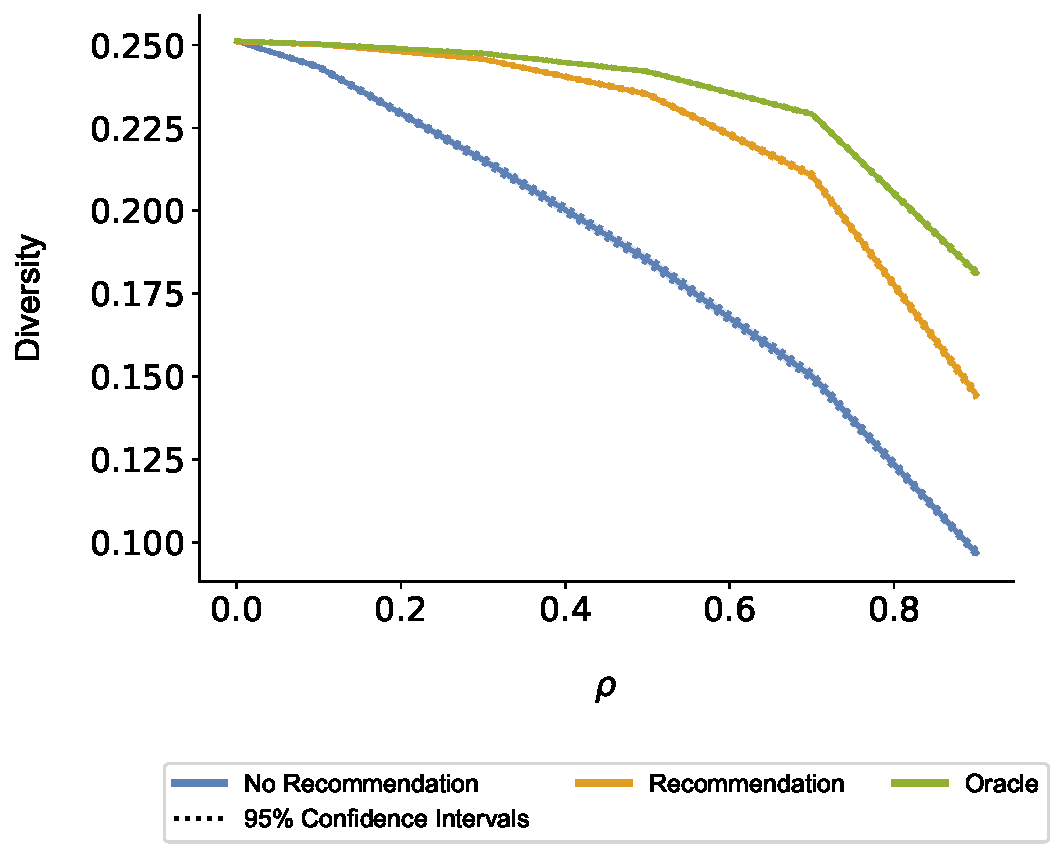
\includegraphics[width=.8\linewidth]{figures/rho_diversity_N_200_T_20.pdf}
\end{subfigure}
\ContinuedFloat
\begin{subfigure}{.45\linewidth}
  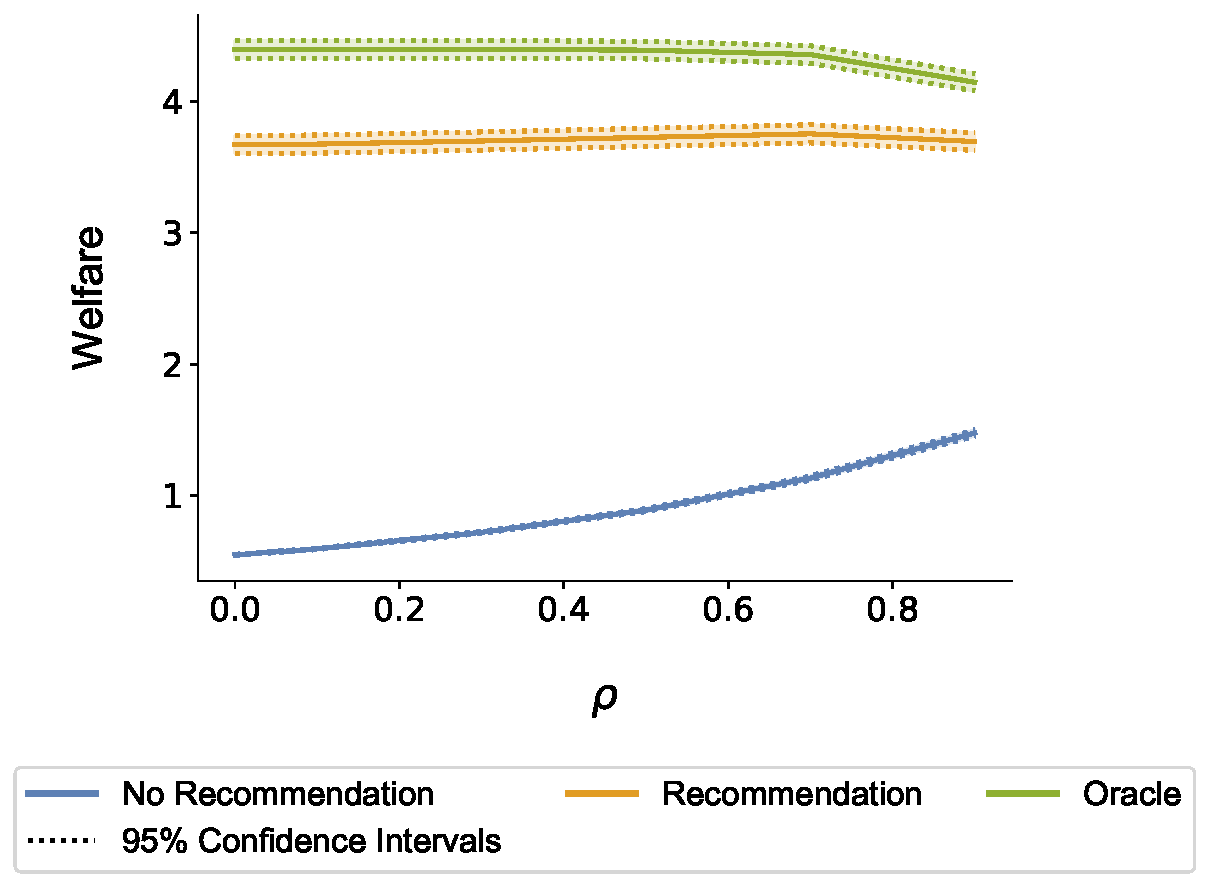
\includegraphics[width=.8\linewidth]{figures/rho_welfare_N_200_T_20.pdf}
\end{subfigure}
\caption*{\scriptsize Notes: The figure on the left displays the relationship between $rho$, the correlation between valuations of items, and overall consumed product diversity. The figure on the right displays the relationship between $\rho$ and overall welfare.}
\end{figure}

\addtocounter{figure}{-1}

\begin{figure}[ht]
\caption{Relationship between $\rho$ and Homogeneity, $N = 200$}
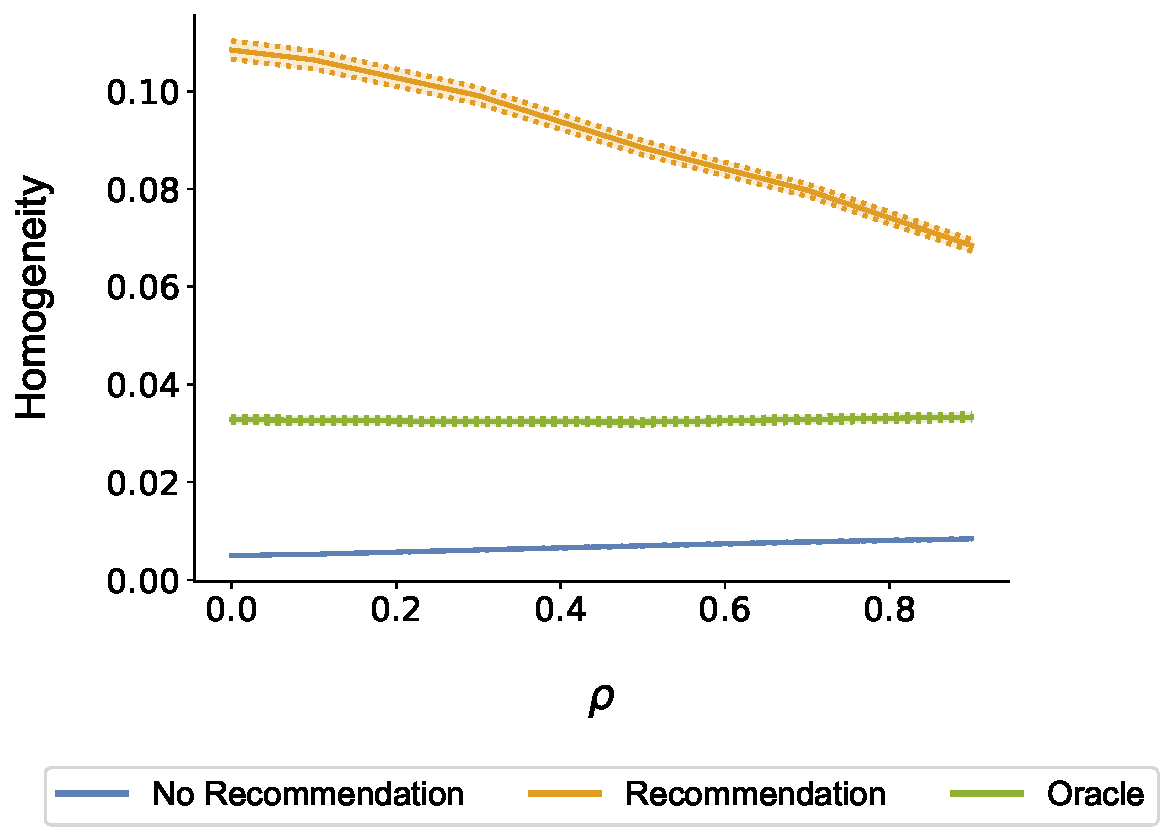
\includegraphics[width=.45\linewidth]{figures/rho_homogeneity_N_200_T_20}
\caption*{\scriptsize Notes: Notes: This figure displays the value of the homogeneity measure as we vary the inherent correlation between the valuation of the items, $\rho$. Each line represents this plot for a single recommendation regime.}\label{fig:cor_homo}
\end{figure}

\begin{figure}[H]
\caption{Relationship between Local Consumption and $\rho$, $N = 200$}
\begin{subfigure}{.45\textwidth}
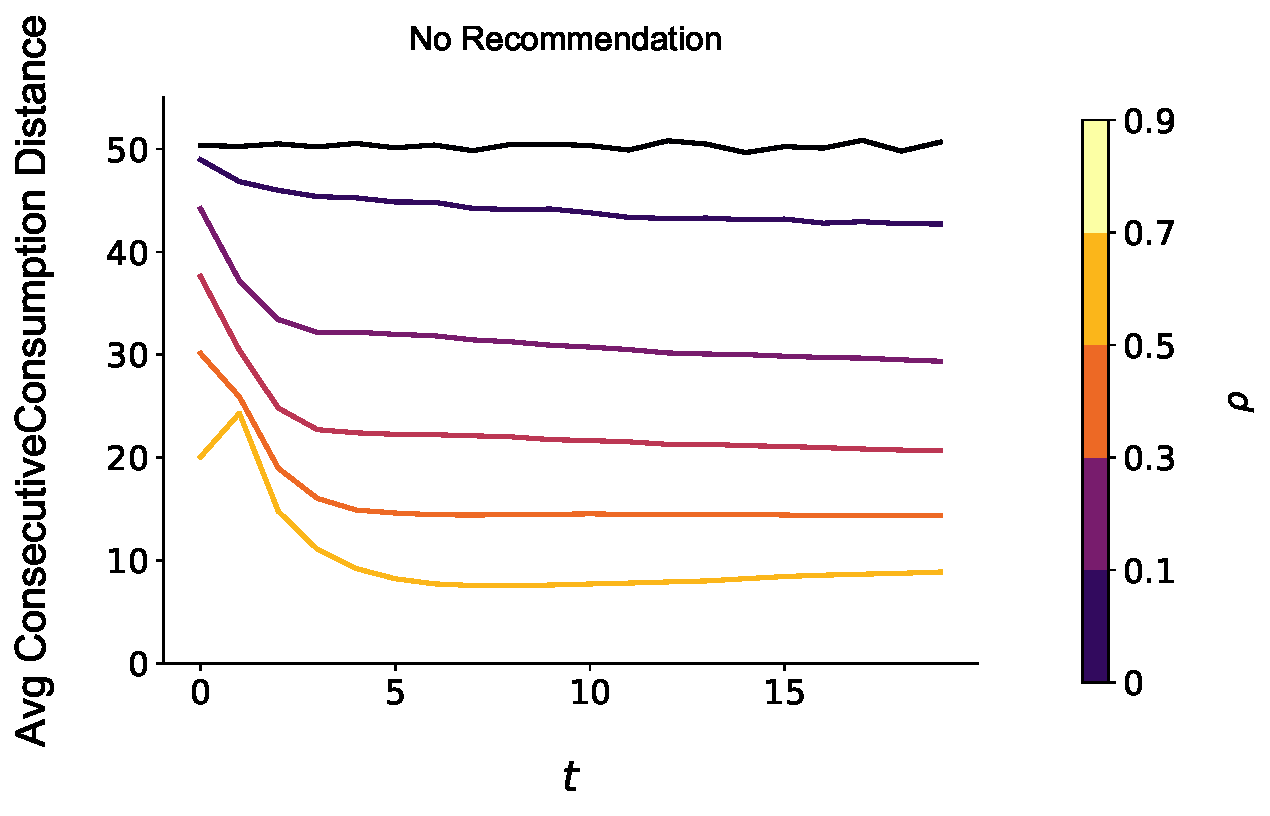
\includegraphics[width=\linewidth]{figures/rho_consumption_dist_N_200T_20.pdf}
\end{subfigure}
\begin{subfigure}{.45\textwidth}
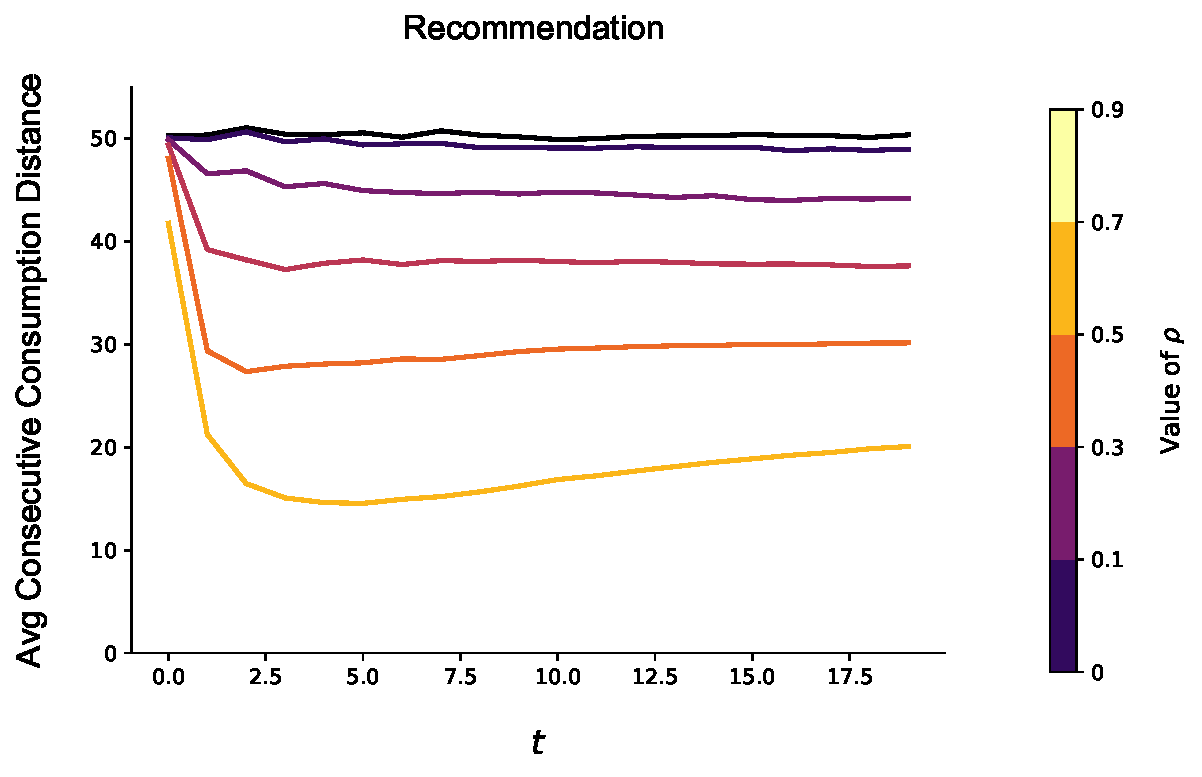
\includegraphics[width=\linewidth]{figures/rho_consumption_dist_N_200T_20_partial.pdf}
\end{subfigure}\\
\begin{subfigure}{.45\textwidth}
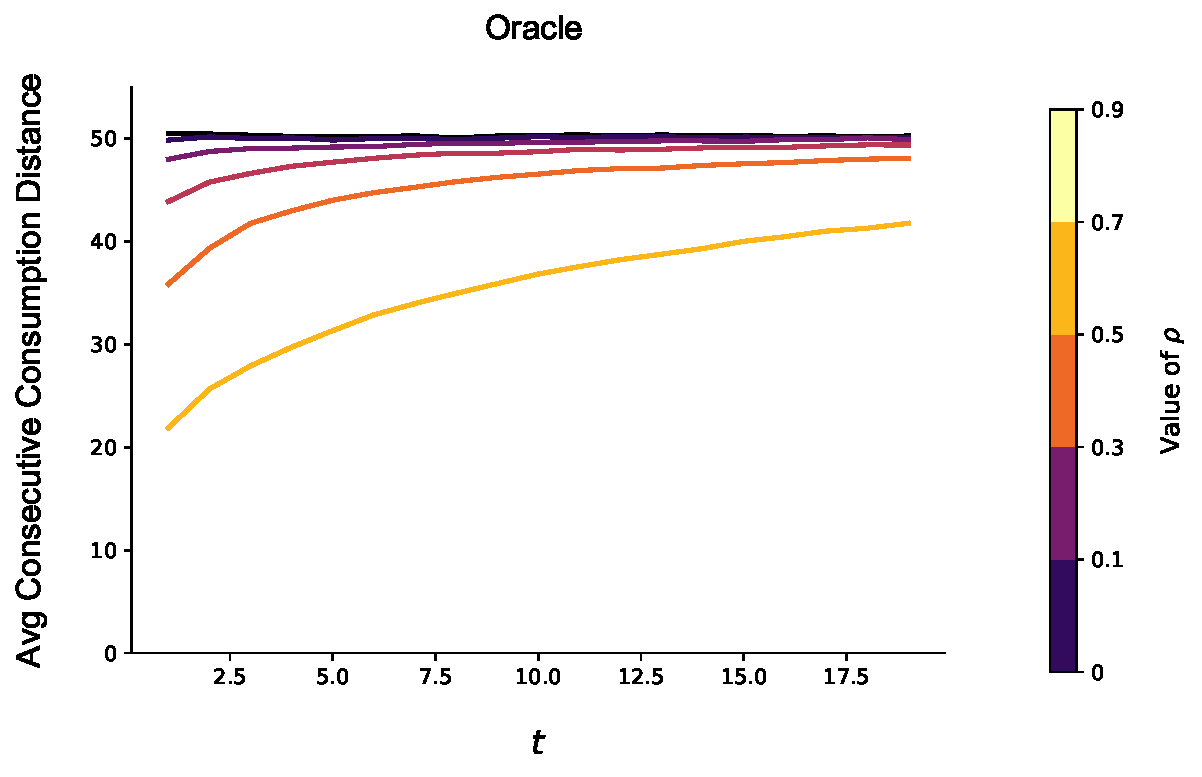
\includegraphics[width=\linewidth]{figures/rho_consumption_dist_N_200T_20_omni.pdf}\\
\end{subfigure}
\caption*{\scriptsize Notes: Each figure plots the average consecutive consumption distance across time as the inherent correlation between the valuation of the items, $\rho$. The top left displays the no recommendation regime, the top right displays the recommendation regime, and the bottom displays the oracle regime.}
\label{fig:local_consumption_across_rho}
\end{figure}
\addtocounter{figure}{-1}

\begin{figure}[H]
\caption{Relationship between Local Consumption and $\gamma$, $N = 200$}
\begin{subfigure}{.45\textwidth}
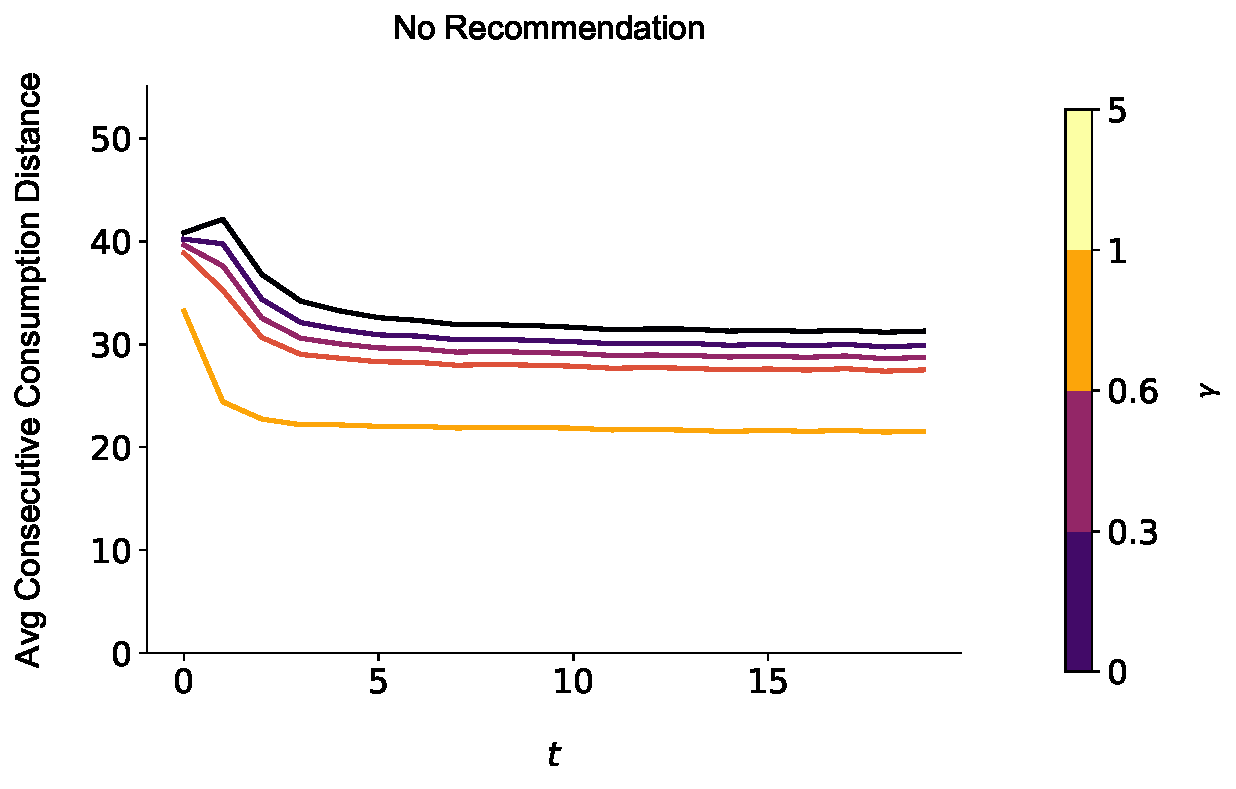
\includegraphics[width=\linewidth]{figures/gamma_consumption_dist_N_200T_20.pdf}
\end{subfigure}
\begin{subfigure}{.45\textwidth}
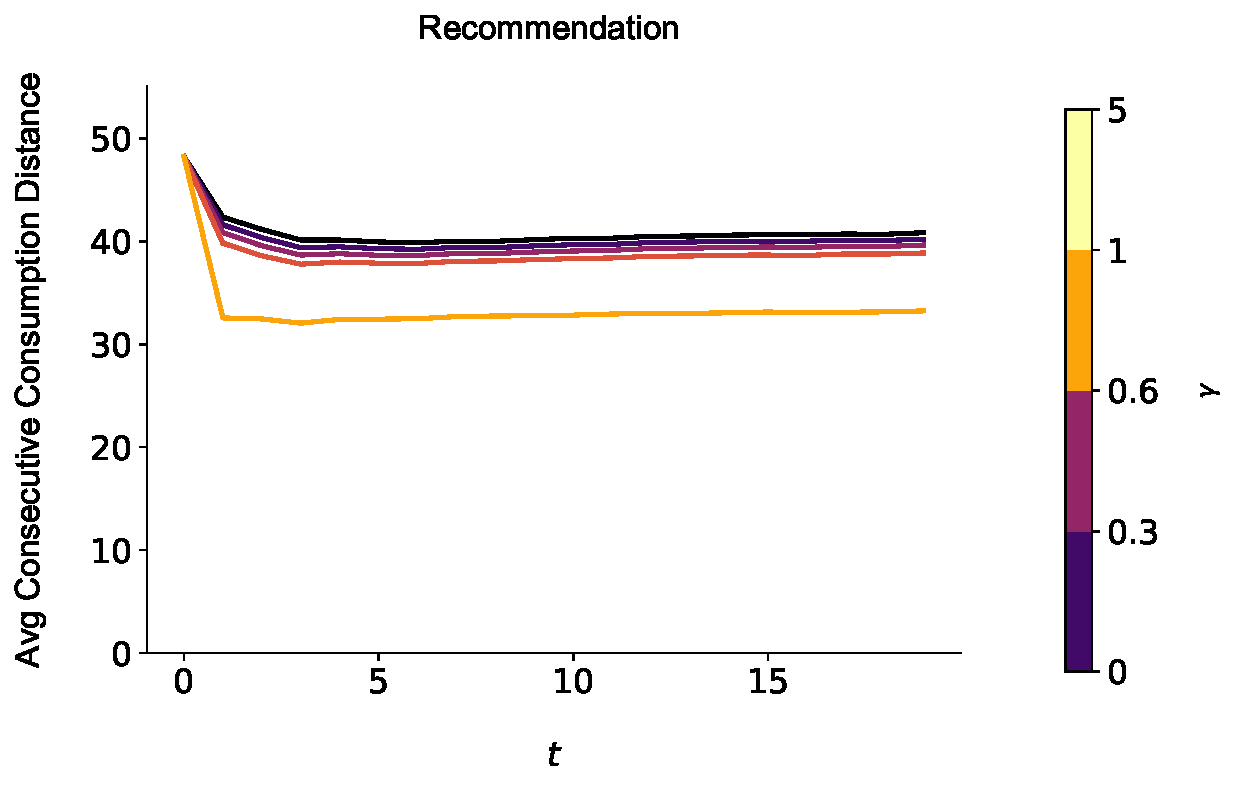
\includegraphics[width=\linewidth]{figures/gamma_consumption_dist_N_200T_20_partial.pdf}
\end{subfigure}\\
\begin{subfigure}{.45\textwidth}
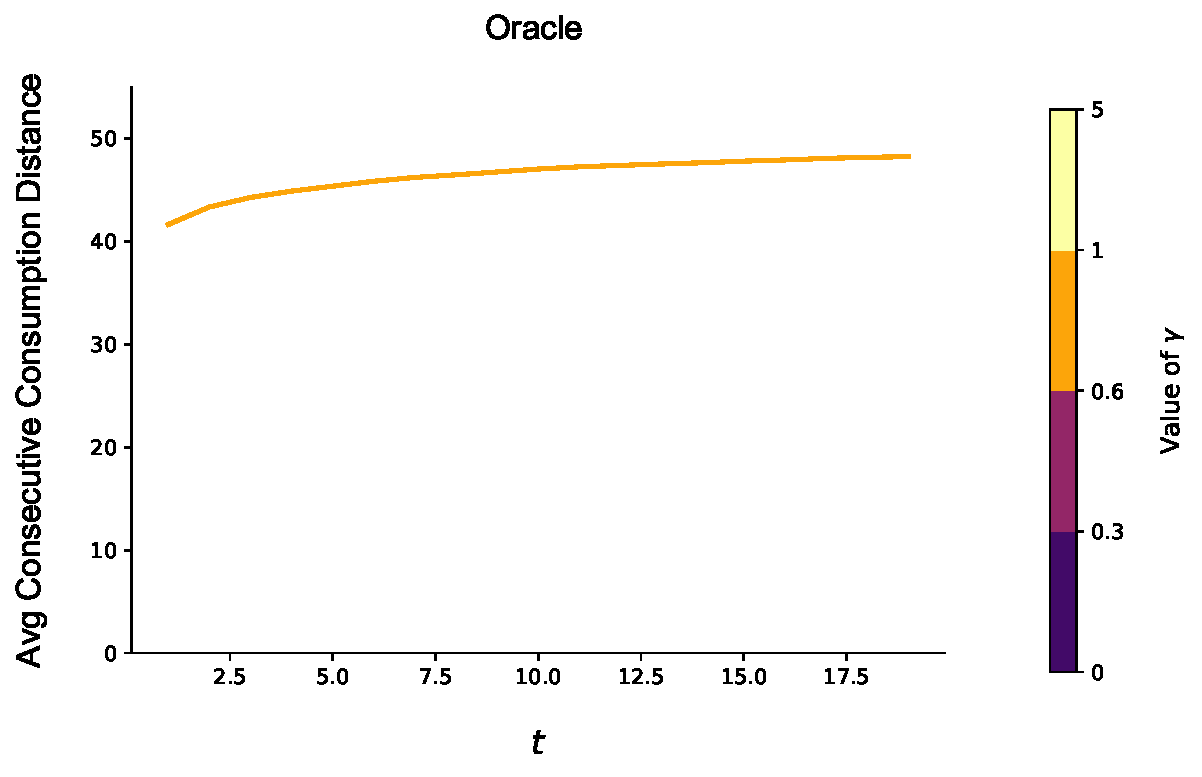
\includegraphics[width=\linewidth]{figures/gamma_consumption_dist_N_200T_20_omni.pdf}\\
\end{subfigure}%
\caption*{\scriptsize Notes: Each figure plots the average consecutive consumption distance across time as the risk aversion level of users, $\gamma$, varies. The top left displays the no recommendation regime, the top right displays the recommendation regime, and the bottom displays the oracle regime.}
\label{fig:no_rec_risk_aversion}
\end{figure}
\addtocounter{figure}{-1}


\clearpage
\section{N = 100}
This section contains the same figures as reported in the main text and appendix, but for $N = 100$ instead of $N = 200$.

\begin{figure}[ht]
\caption{Relationship between $\beta$ and Homogeneity, $N = 100$}
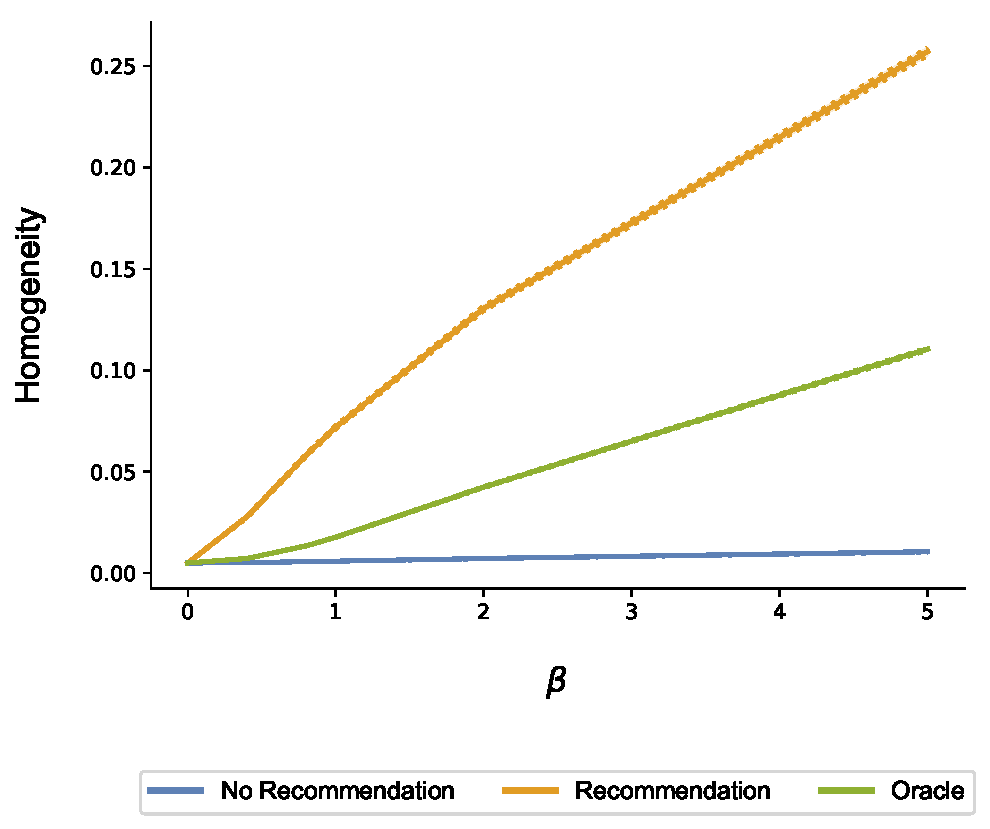
\includegraphics[width=.45\linewidth]{figures/beta_homogeneity_N_200_T_20}\label{fig:beta_homo}
\caption*{\scriptsize Notes: This figure displays the value of the homogeneity measure as we vary the weight of the common value component, $\beta$. Each line represents this plot for a single recommendation regime.}
\end{figure}
\begin{figure}[ht]
\caption{Relationship between $\rho$ and Homogeneity, $N = 100$}
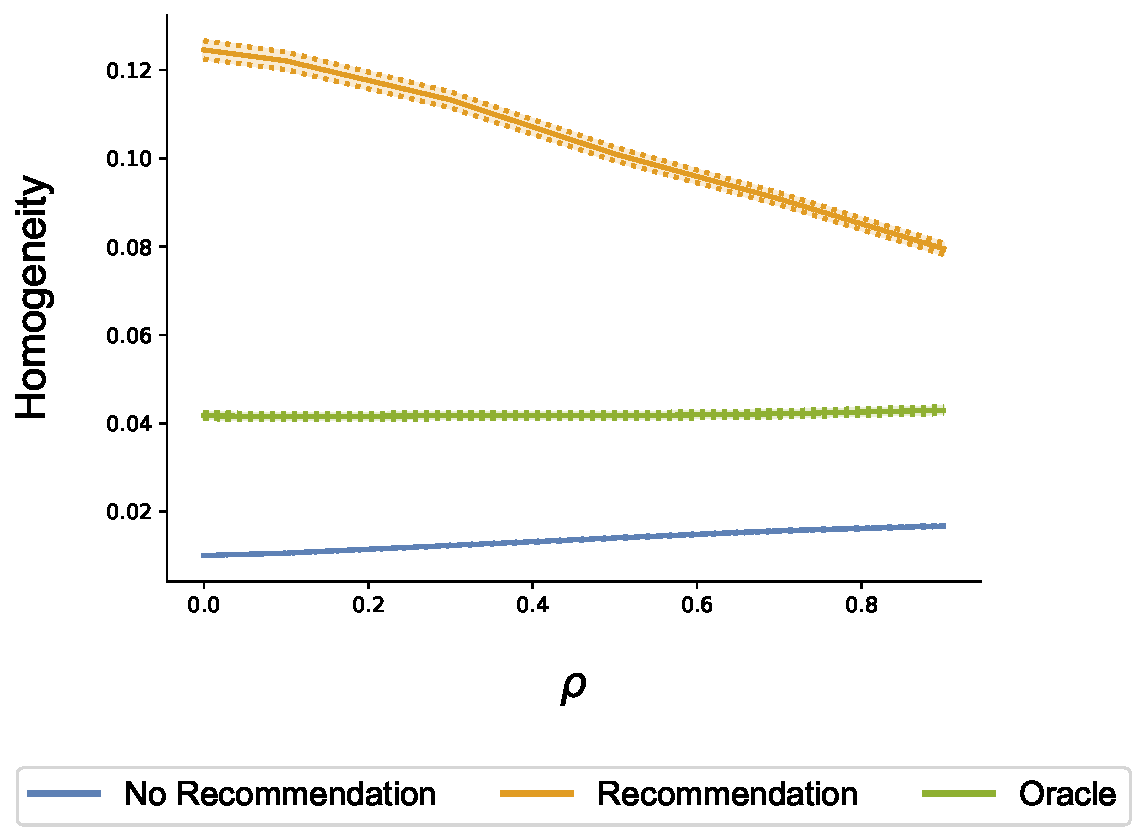
\includegraphics[width=.45\linewidth]{figures/rho_homogeneity_N_100_T_20}
\caption*{\scriptsize Notes: Notes: This figure displays the value of the homogeneity measure as we vary the inherent correlation between the valuation of the items, $\rho$. Each line represents this plot for a single recommendation regime.}\label{fig:cor_homo}
\end{figure}

\begin{figure}[H]
\caption{Relationship between Local Consumption and $\gamma$, $N = 100$}
\begin{subfigure}{.45\textwidth}
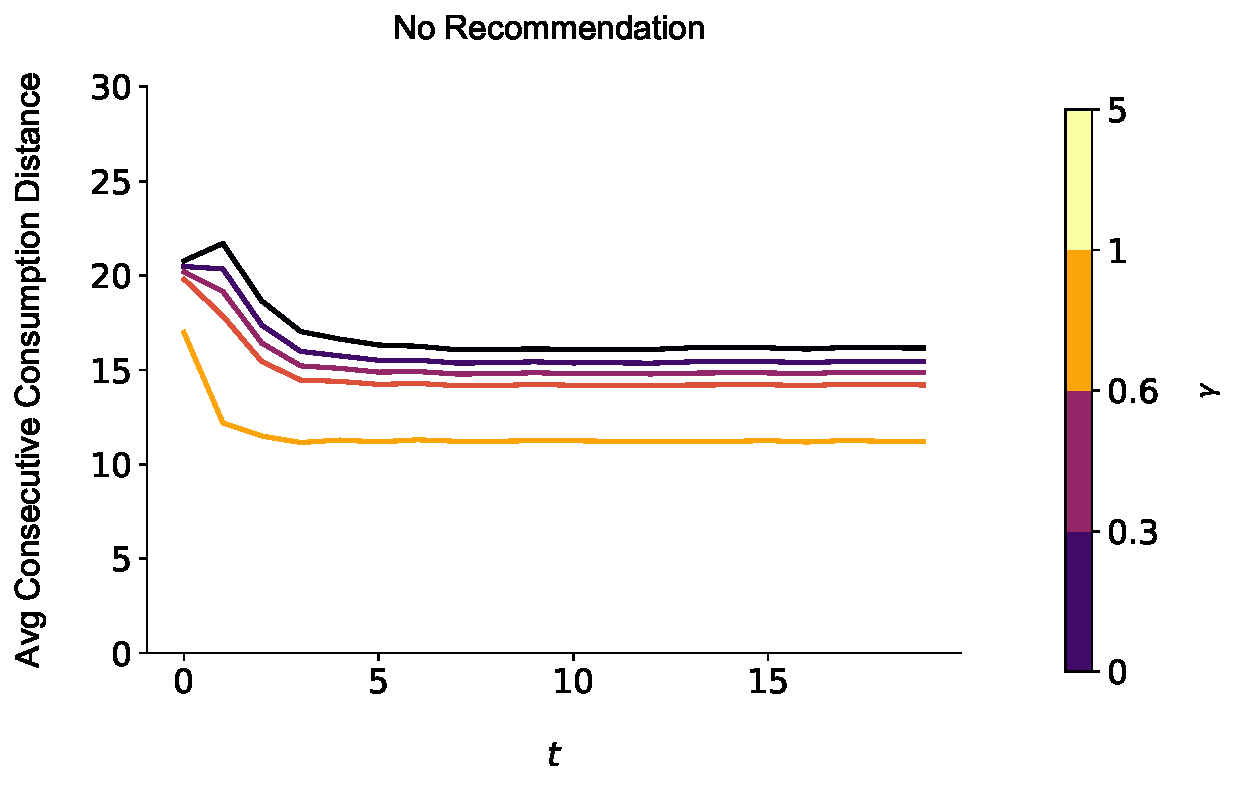
\includegraphics[width=\linewidth]{figures/gamma_consumption_dist_N_100T_20.pdf}
\end{subfigure}
\begin{subfigure}{.45\textwidth}
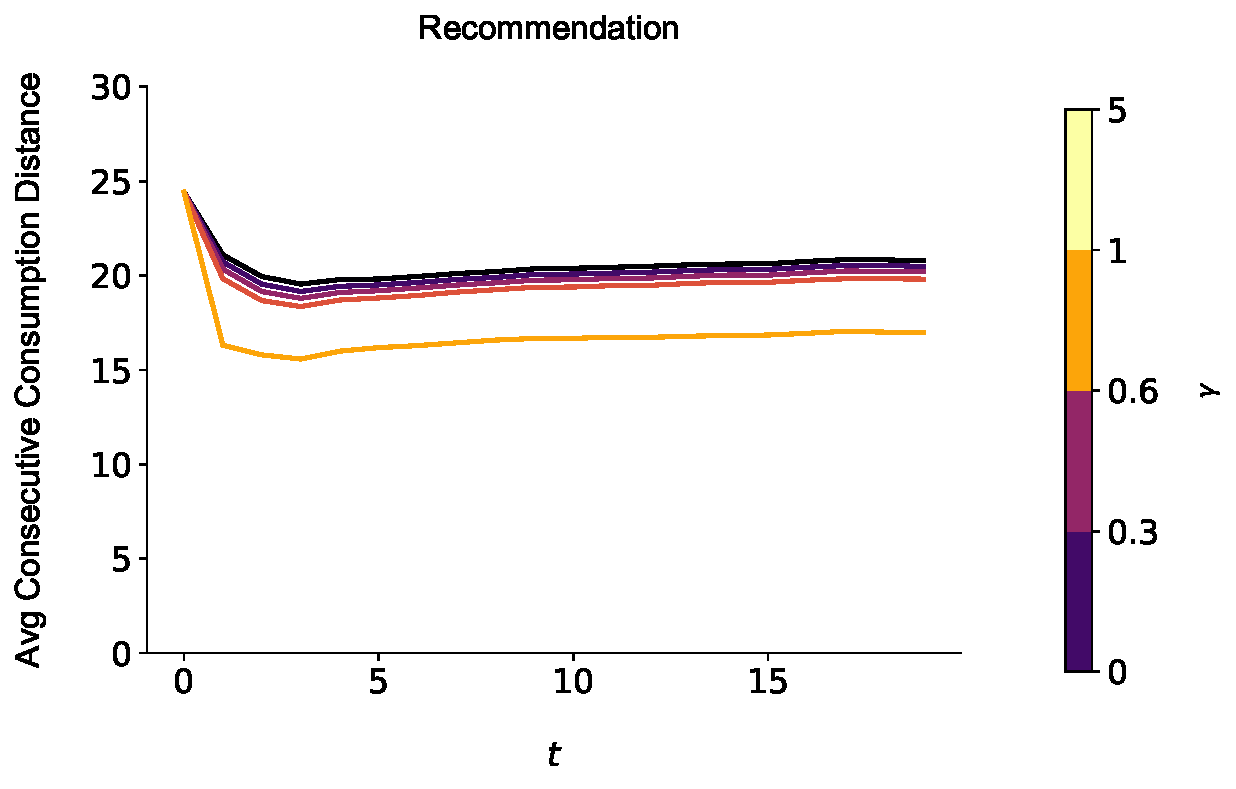
\includegraphics[width=\linewidth]{figures/gamma_consumption_dist_N_100T_20_partial.pdf}
\end{subfigure}\\
\begin{subfigure}{.45\textwidth}
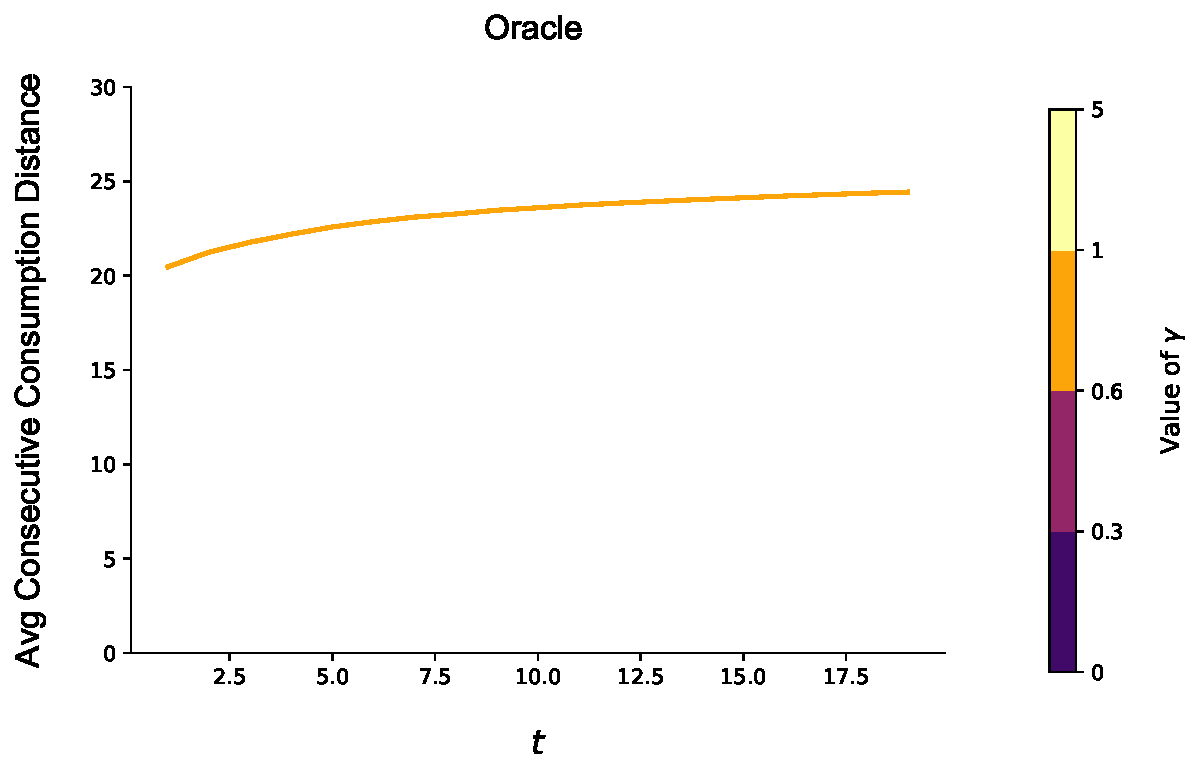
\includegraphics[width=\linewidth]{figures/gamma_consumption_dist_N_100T_20_omni.pdf}\\
\end{subfigure}%
\caption*{\scriptsize Notes: Each figure plots the average consecutive consumption distance across time as the risk aversion level of users, $\gamma$, varies. The top left displays the no recommendation regime, the top right displays the recommendation regime, and the bottom displays the oracle regime.}
\label{fig:no_rec_risk_aversion}
\end{figure}
\addtocounter{figure}{-1}

\begin{figure}[H]
\caption{Local Consumption and Correlation, $N = 100$}
\begin{subfigure}{.5\linewidth}
  \centering
  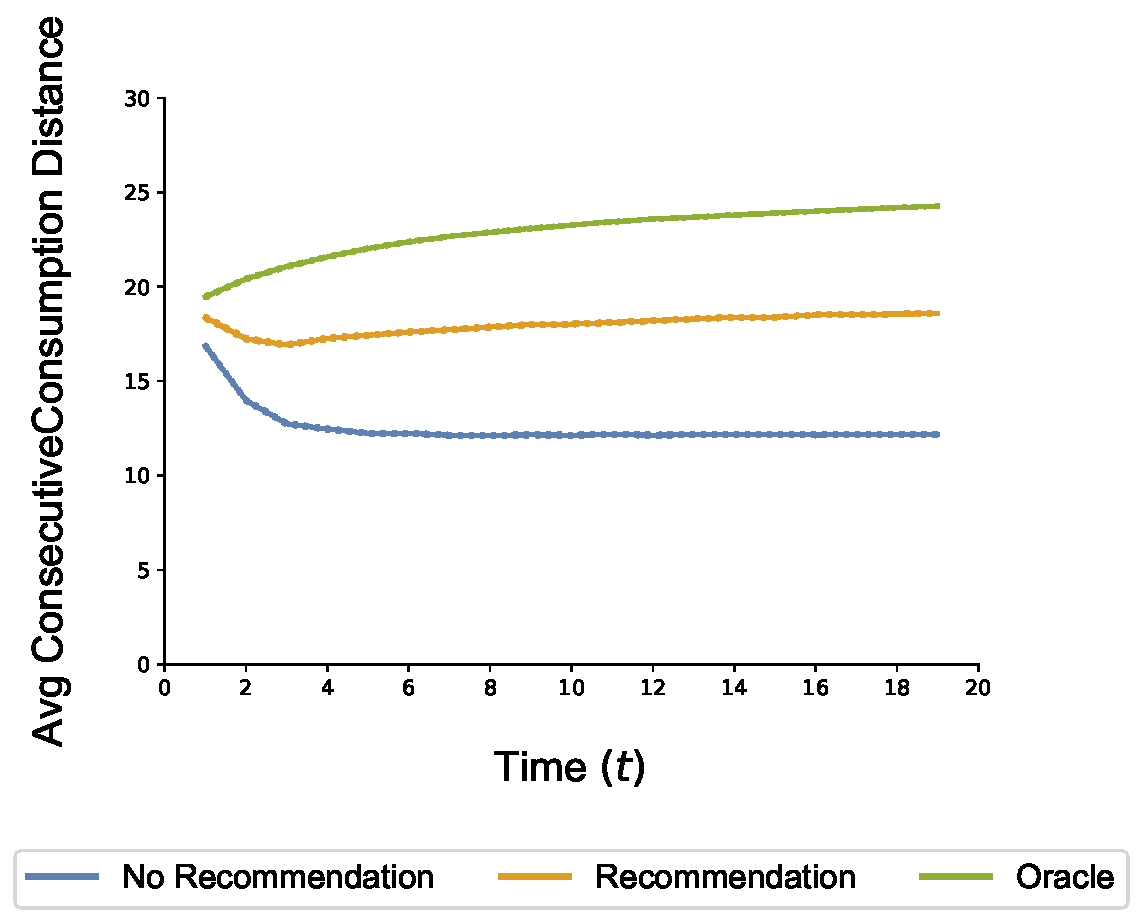
\includegraphics[width=.9\linewidth]{figures/rho_pos_consumption_dist_N_100T_20_overall.pdf}
  \label{fig:sfig1}
\end{subfigure}%
\begin{subfigure}{.5\linewidth}
  \centering
  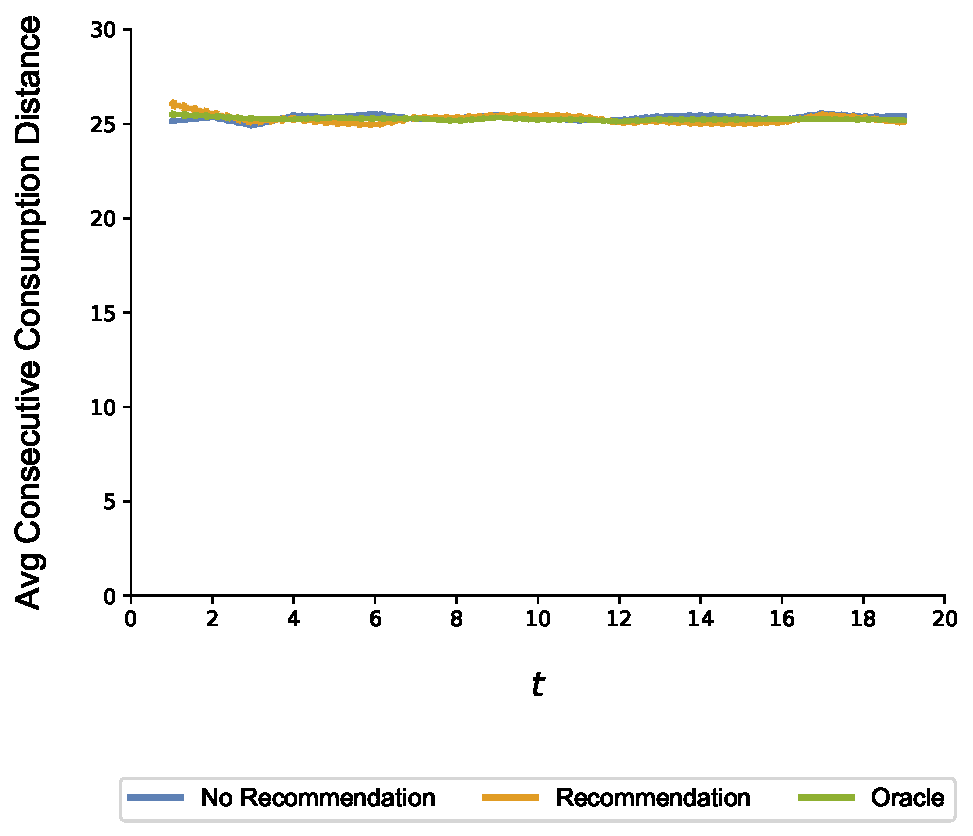
\includegraphics[width=.9\linewidth]{figures/rho_zero_consumption_dist_N_100T_20_overall.pdf}
  \label{fig:sfig2}
\end{subfigure}
\caption*{\footnotesize Notes: The figure shows the consecutive consumption path difference between the no recommendation, recommendation, and oracle regime. The figure on the left displays the average consecutive consumption distance aggregating over simulations where $\rho = 0$ and the figure on the right displays the average consecutive consumption distance aggregating over simulations where $\rho > 0$}
\label{fig:correlation_consumption_path_n_100}
\end{figure}
\addtocounter{figure}{-1}


% Paper body
\begin{figure}[H]
\captionof{figure}{Relationship between Local Consumption and $\rho$, $N = 100$}
\begin{subfigure}{.45\textwidth}
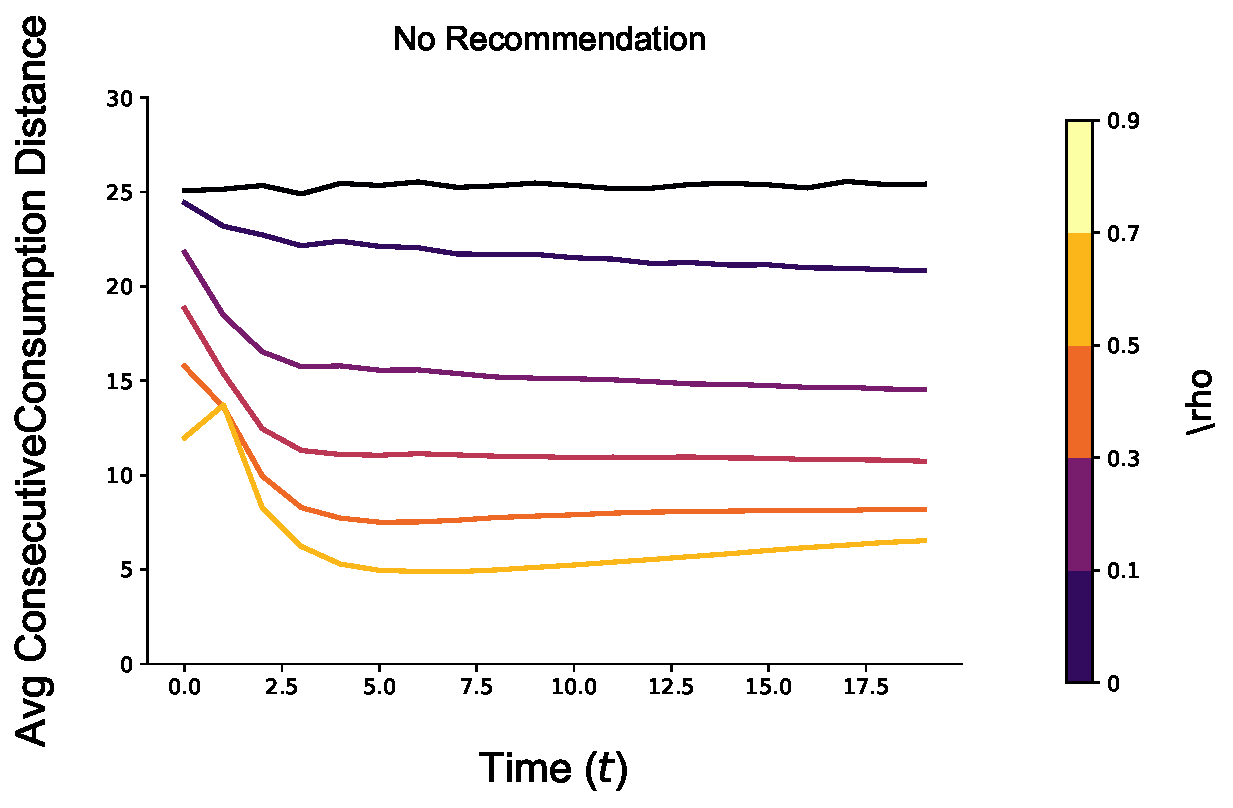
\includegraphics[width=\linewidth]{figures/rho_consumption_dist_N_100T_20.pdf}
\end{subfigure}
\begin{subfigure}{.45\textwidth}
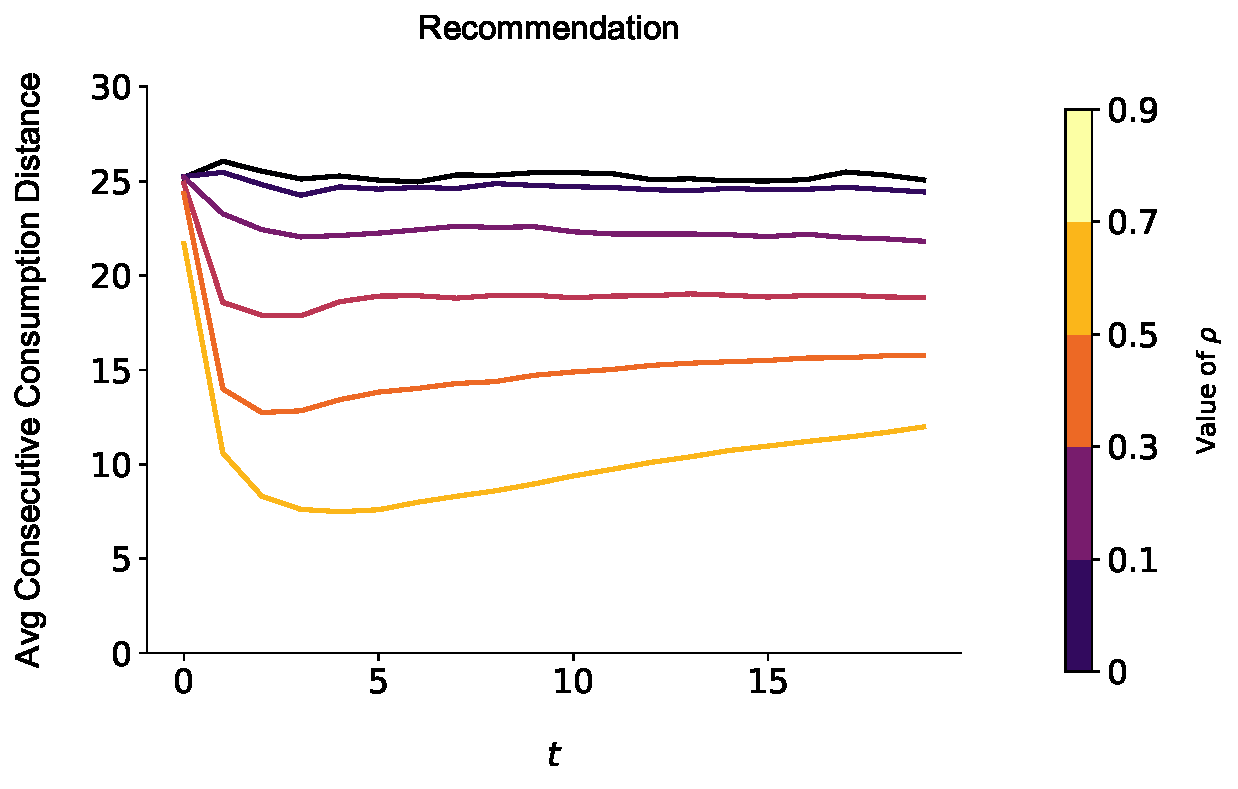
\includegraphics[width=\linewidth]{figures/rho_consumption_dist_N_100T_20_partial.pdf}
\end{subfigure}\\
\begin{subfigure}{.45\textwidth}
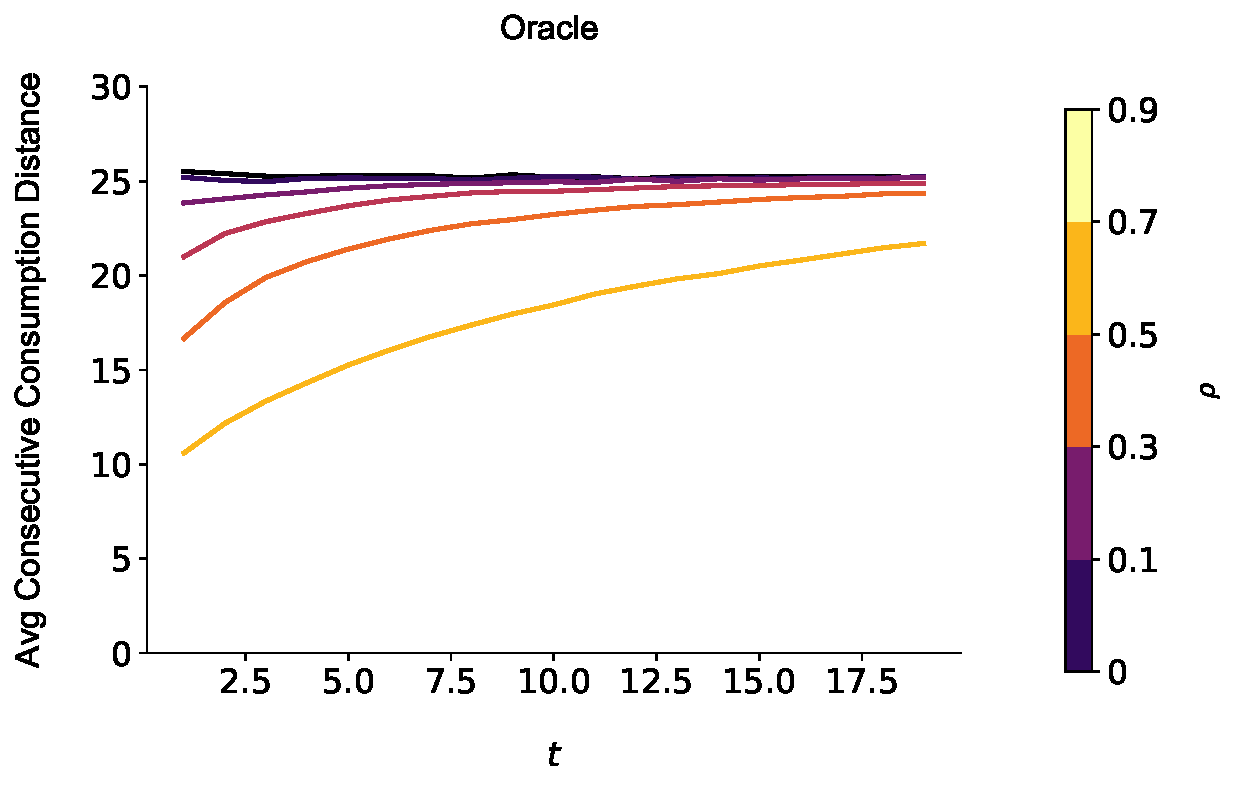
\includegraphics[width=\linewidth]{figures/rho_consumption_dist_N_100T_20_omni.pdf}\\
\end{subfigure}
\caption*{\scriptsize Notes: Each figure plots the average consecutive consumption distance across time as the inherent correlation between the valuation of the items, $\rho$. The top left displays the no recommendation regime, the top right displays the recommendation regime, and the bottom displays the oracle regime.}
\label{fig:local_consumption_across_rho}
\end{figure}

\clearpage

\section{N = 500}

This section contains the same figures as reported in the main text and appendix, but for $N = 500$ instead of $N = 200$.

\begin{figure}[ht]
\caption{Relationship between $\beta$ and Homogeneity, $N = 500$}
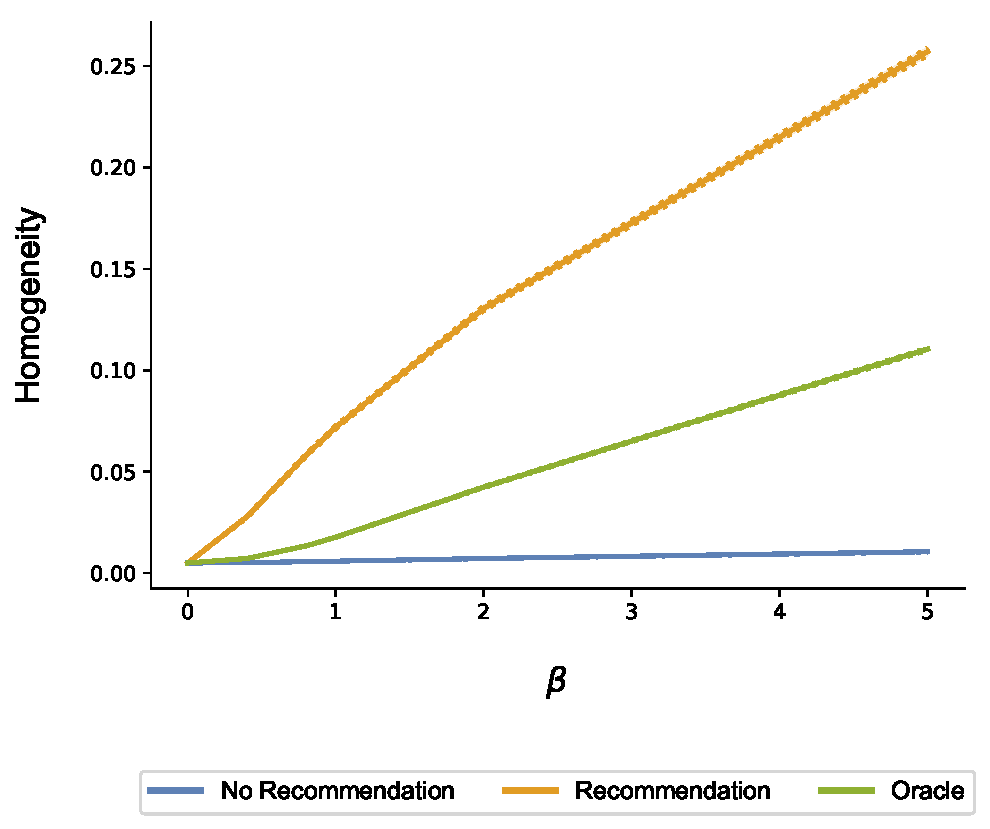
\includegraphics[width=.45\linewidth]{figures/beta_homogeneity_N_200_T_20}\label{fig:beta_homo}
\caption*{\scriptsize Notes: This figure displays the value of the homogeneity measure as we vary the weight of the common value component, $\beta$. Each line represents this plot for a single recommendation regime.}
\end{figure}
\begin{figure}[ht]
\caption{Relationship between $\rho$ and Homogeneity, $N = 500$}
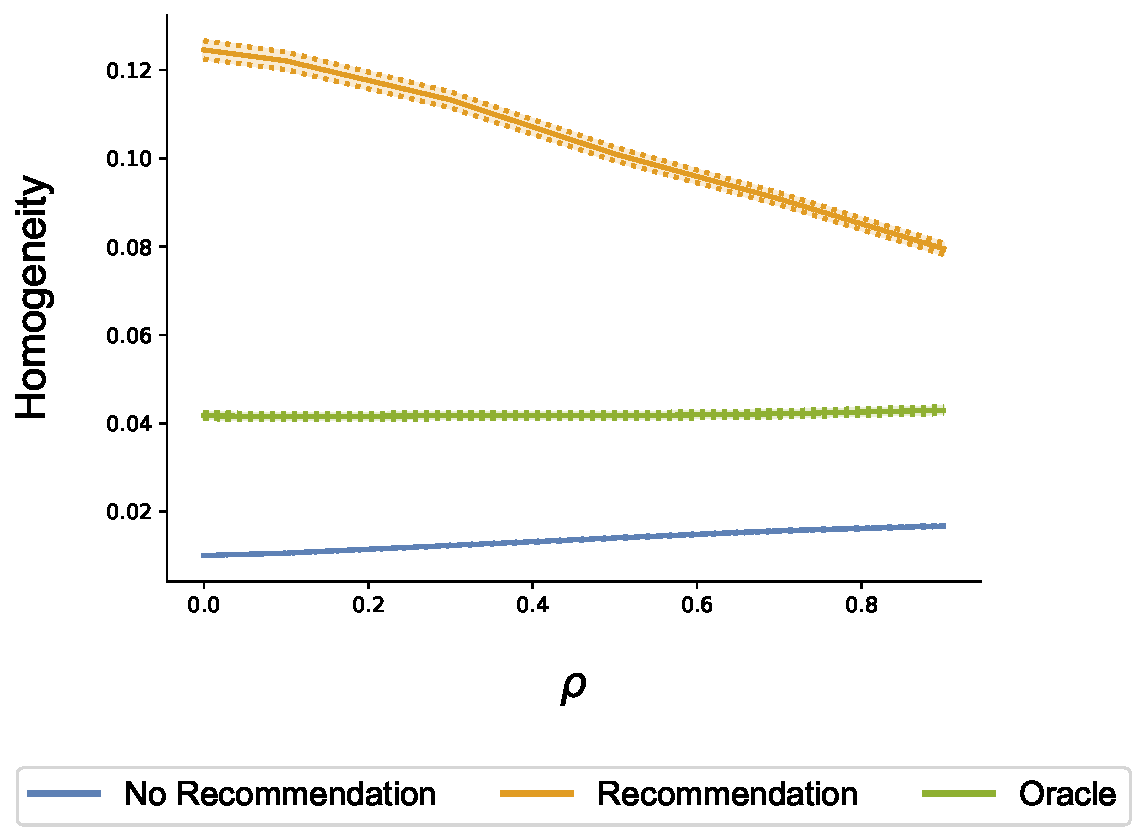
\includegraphics[width=.45\linewidth]{figures/rho_homogeneity_N_100_T_20}
\caption*{\scriptsize Notes: Notes: This figure displays the value of the homogeneity measure as we vary the inherent correlation between the valuation of the items, $\rho$. Each line represents this plot for a single recommendation regime.}\label{fig:cor_homo}
\end{figure}

\begin{figure}[H]
\captionof{figure}{Relationship between Local Consumption and $\gamma$, $N = 500$}
\begin{subfigure}{.45\textwidth}
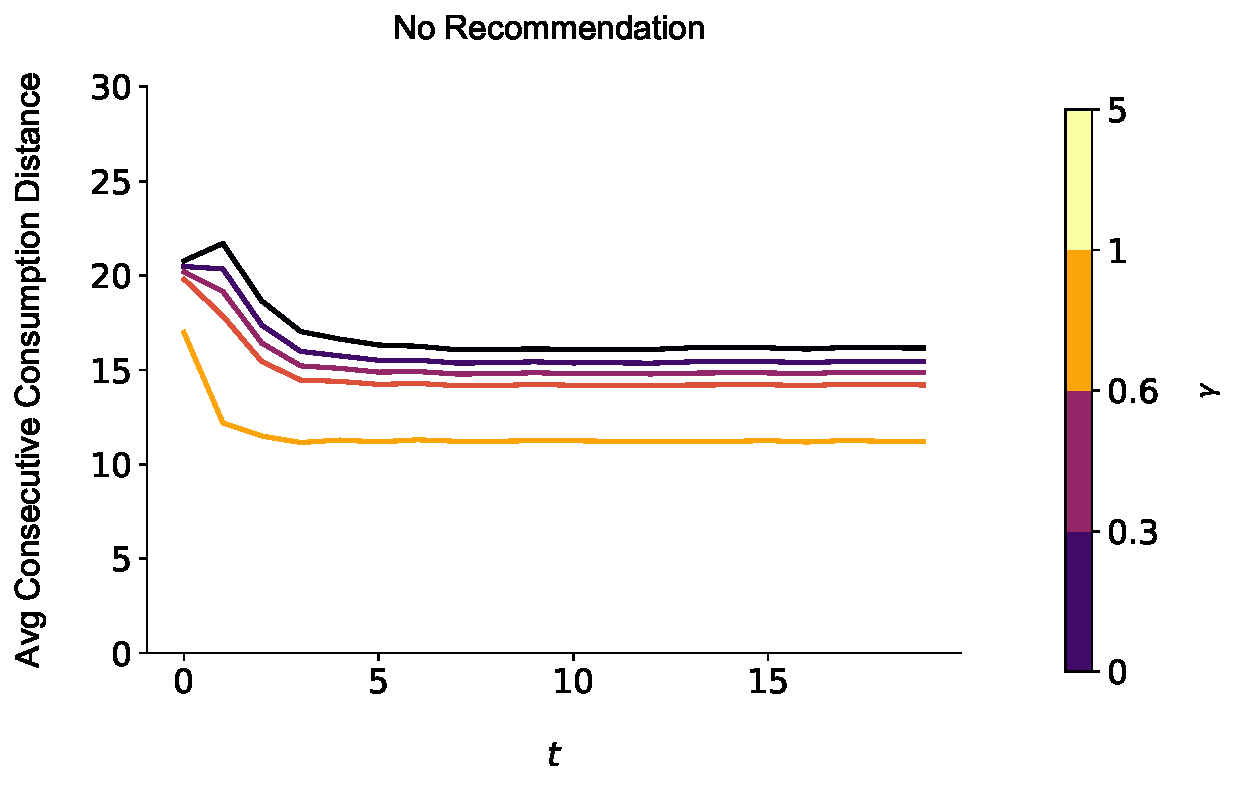
\includegraphics[width=\linewidth]{figures/gamma_consumption_dist_N_100T_20.pdf}
\end{subfigure}
\begin{subfigure}{.45\textwidth}
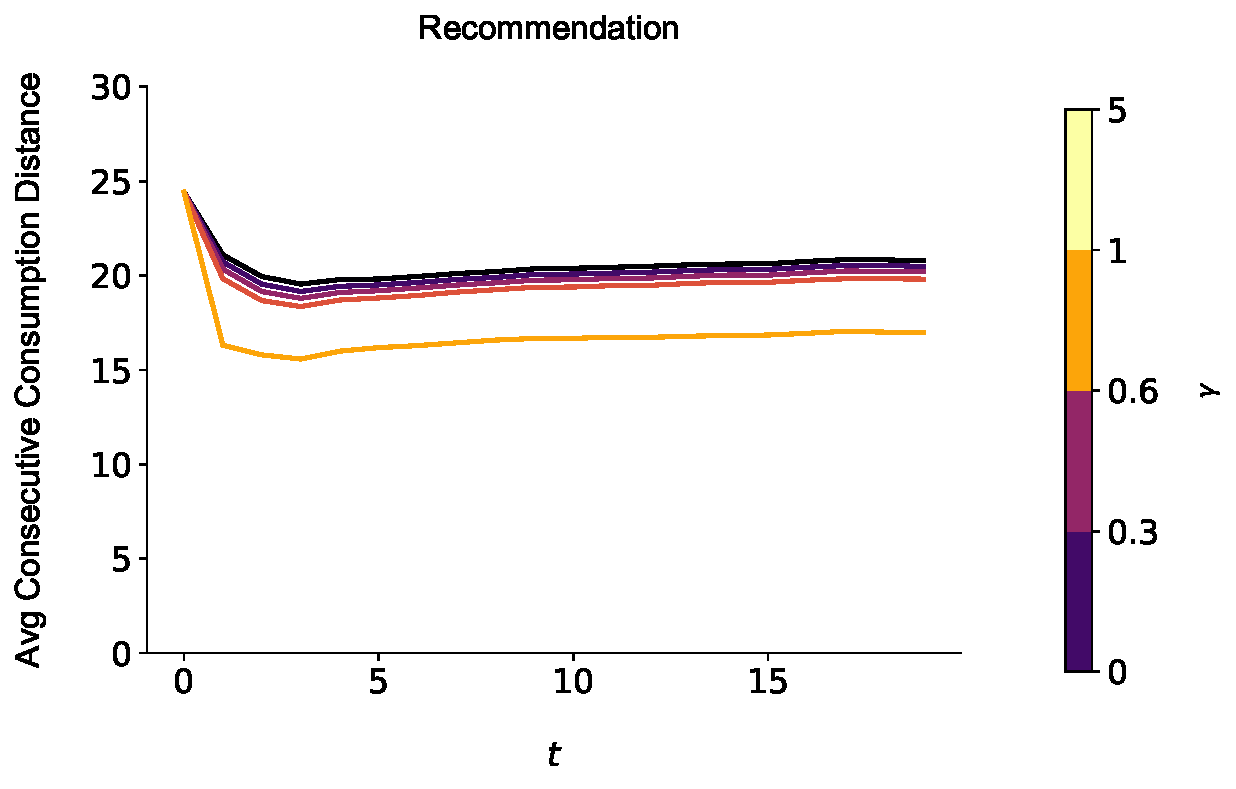
\includegraphics[width=\linewidth]{figures/gamma_consumption_dist_N_100T_20_partial.pdf}
\end{subfigure}\\
\begin{subfigure}{.45\textwidth}
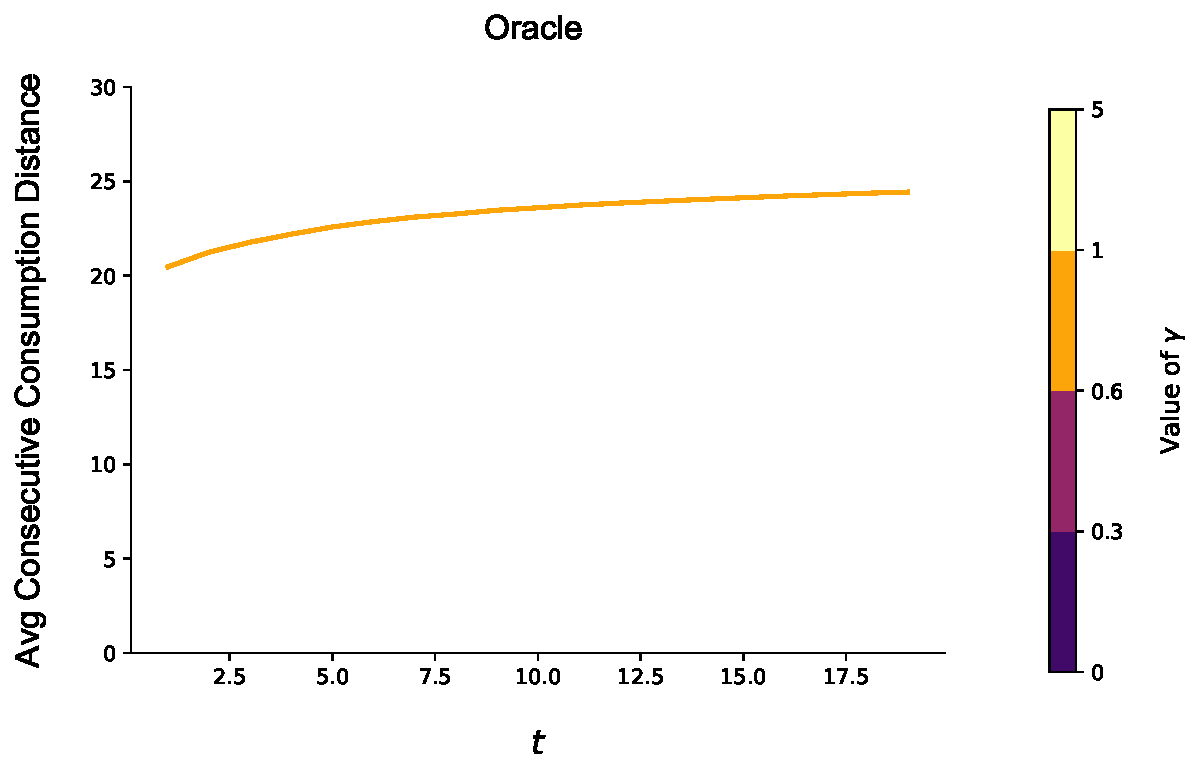
\includegraphics[width=\linewidth]{figures/gamma_consumption_dist_N_100T_20_omni.pdf}\\
\end{subfigure}%
\caption*{\scriptsize Notes: Each figure plots the average consecutive consumption distance across time as the risk aversion level of users, $\gamma$, varies. The top left displays the no recommendation regime, the top right displays the recommendation regime, and the bottom displays the oracle regime.}
\label{fig:no_rec_risk_aversion}
\end{figure}

\addtocounter{figure}{-1}

% Paper body
\begin{figure}[H]
\caption{Relationship between Local Consumption and $\rho$, $N = 500$}
\begin{subfigure}{.45\textwidth}
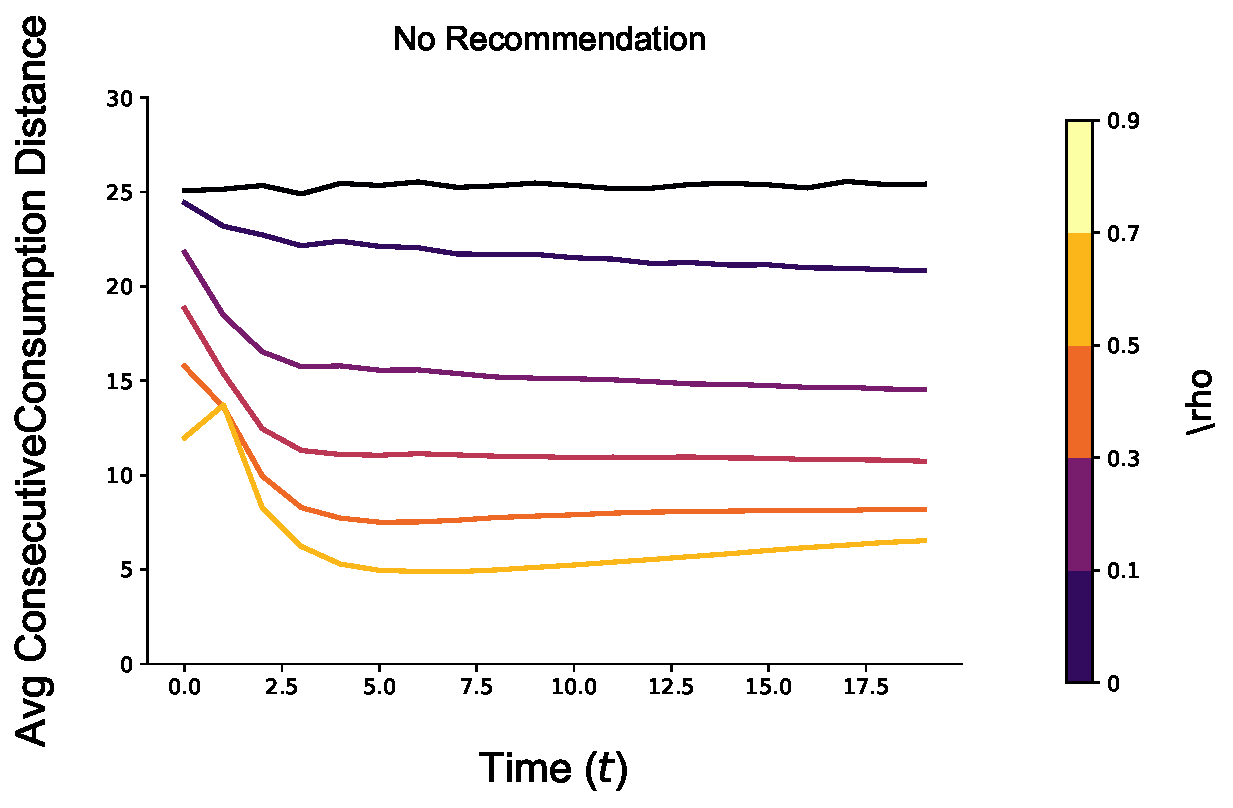
\includegraphics[width=\linewidth]{figures/rho_consumption_dist_N_100T_20.pdf}
\end{subfigure}
\begin{subfigure}{.45\textwidth}
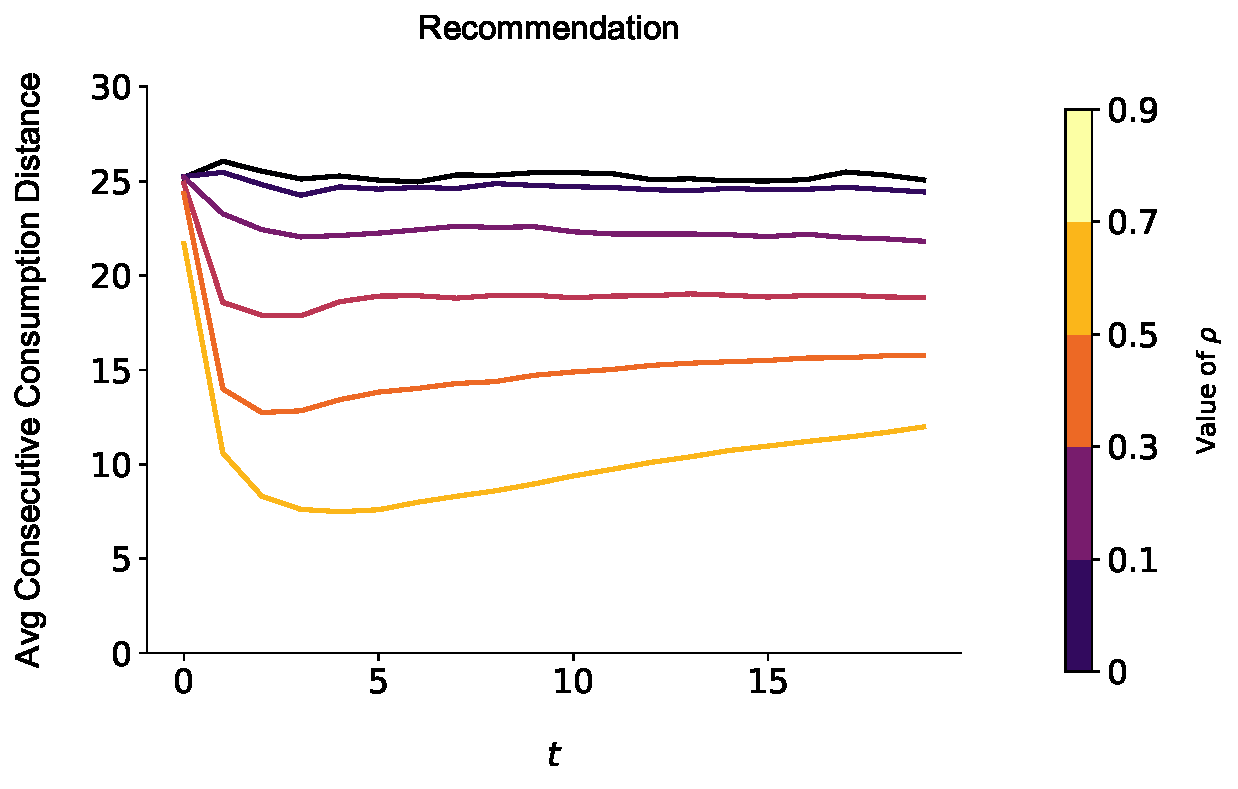
\includegraphics[width=\linewidth]{figures/rho_consumption_dist_N_100T_20_partial.pdf}
\end{subfigure}\\
\begin{subfigure}{.45\textwidth}
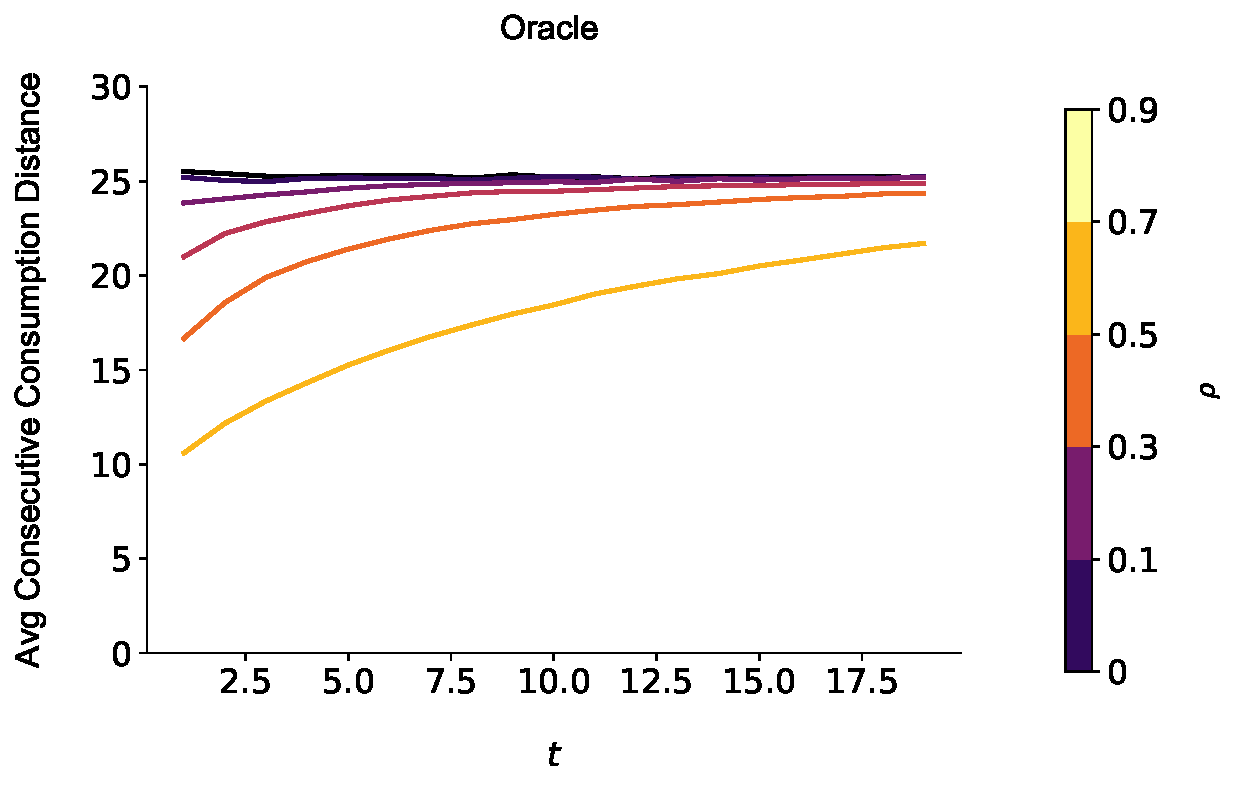
\includegraphics[width=\linewidth]{figures/rho_consumption_dist_N_100T_20_omni.pdf}\\
\end{subfigure}
\caption*{\scriptsize Notes: Each figure plots the average consecutive consumption distance across time as the inherent correlation between the valuation of the items, $\rho$. The top left displays the no recommendation regime, the top right displays the recommendation regime, and the bottom displays the oracle regime.}
\label{fig:local_consumption_across_rho}
\end{figure}

\addtocounter{figure}{-1}

\begin{figure}[H]
\caption{Local Consumption and Correlation, $N = 500$}
\begin{subfigure}{.5\linewidth}
  \centering
  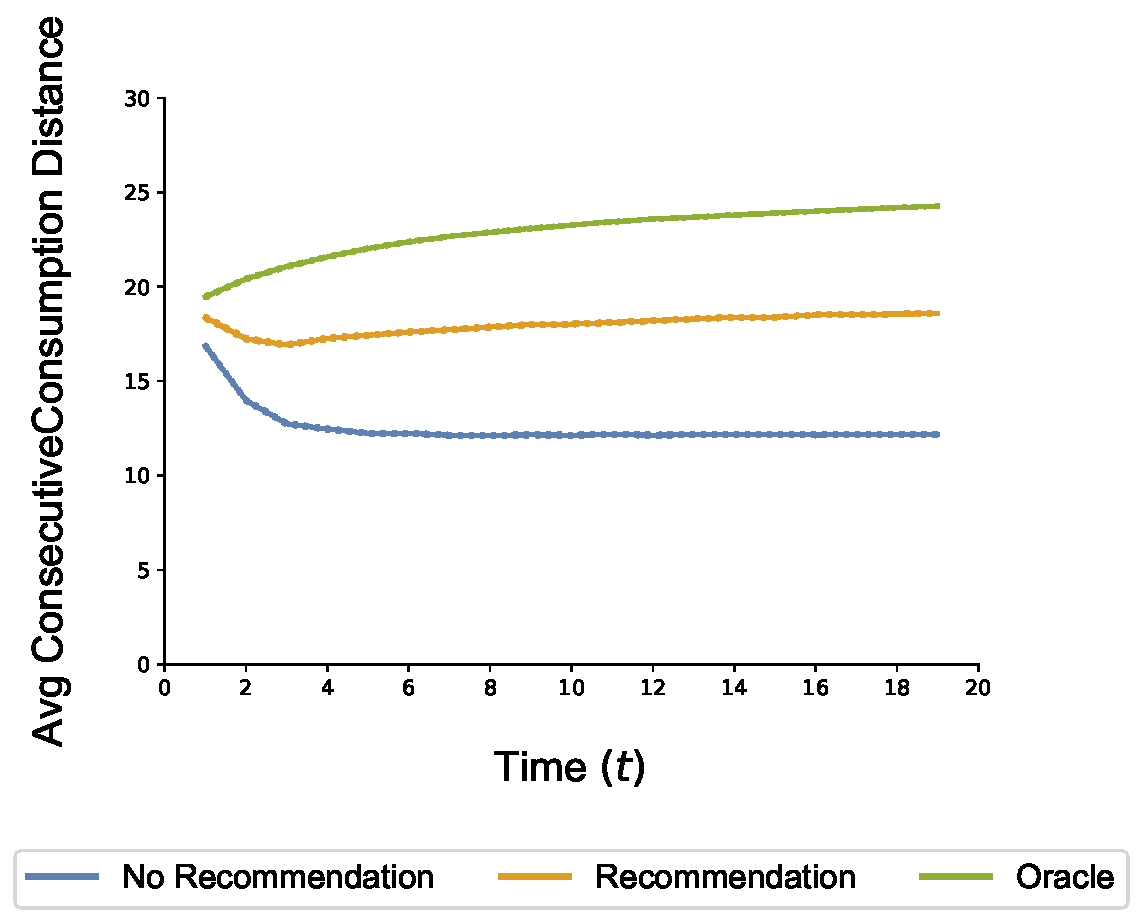
\includegraphics[width=.9\linewidth]{figures/rho_pos_consumption_dist_N_100T_20_overall.pdf}
  \label{fig:sfig1}
\end{subfigure}%
\begin{subfigure}{.5\linewidth}
  \centering
  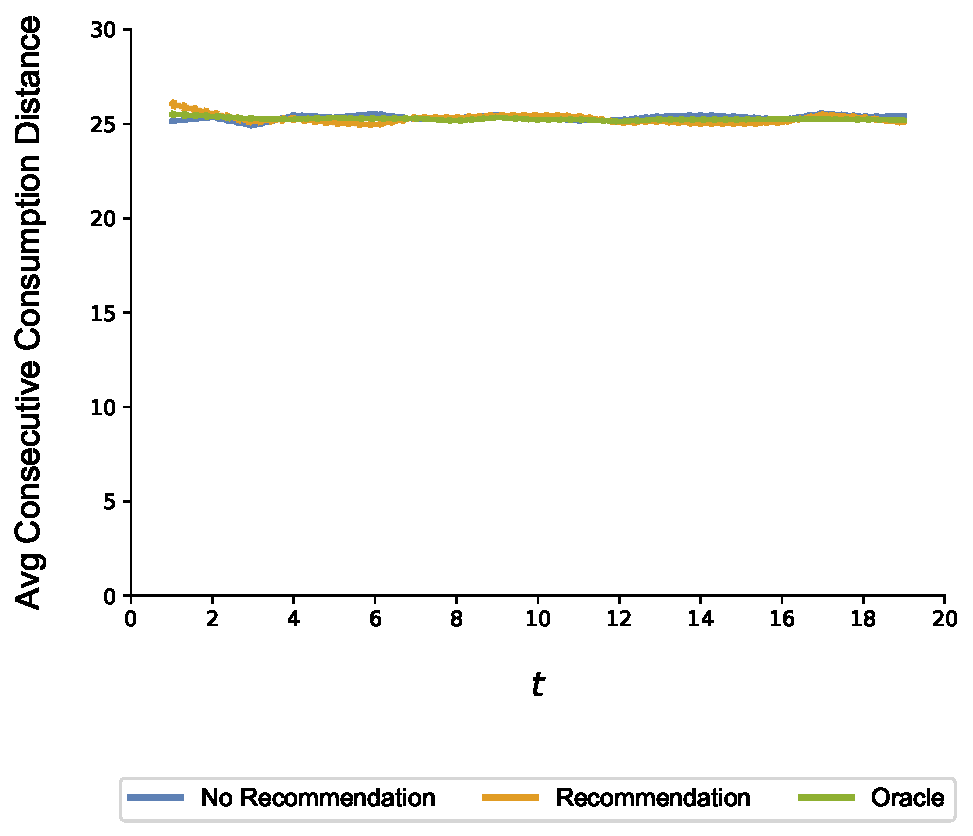
\includegraphics[width=.9\linewidth]{figures/rho_zero_consumption_dist_N_100T_20_overall.pdf}
  \label{fig:sfig2}
\end{subfigure}
\caption*{\scriptsize Notes: The figure shows the consecutive consumption path difference between the no recommendation, recommendation, and oracle regime. The figure on the left displays the average consecutive consumption distance aggregating over simulations where $\rho = 0$ and the figure on the right displays the average consecutive consumption distance aggregating over simulations where $\rho > 0$}
\label{fig:correlation_consumption_path_n_100}
\end{figure}

% Bibliography

\end{document}
